
\documentclass[11pt, aspectratio=169]{beamer}

\usepackage[utf8]{inputenc}
\usepackage{tikz}
\usepackage[english]{babel}
\usepackage{svg}
\usepackage{eurosym}
\usepackage{subfig}
\usepackage{pgfgantt}
\usepackage[export]{adjustbox}
%\usepackage[shortlabels]{enumitem}
\usepackage[font=scriptsize,justification=centering]{caption}

%----------------------------------------------------------------------------------------
%	TITLE PAGE INFORMATION.
%----------------------------------------------------------------------------------------
\author{A. M\"{o}slinger, K. Steele, D. Talavera, N. Ulfvarson, and E.F.M. Weterings}
\title{InfraRed Imaging of astronomical targets with a Stabilised Camera}
\subtitle{IRISC}
\institute{DLR MORABA, Oberpfaffenhofen} 
\date{11-15 February 2019}
%\subject{} 

%----------------------------------------------------------------------------------------
%	SETUP LAYOUT.
%----------------------------------------------------------------------------------------
\usepackage{theme/beamerthemeWarsawLTU}
%\usetheme{Warsaw}


\begin{document}
%----------------------------------------------------------------------------------------
%	TITLE PAGE.
%----------------------------------------------------------------------------------------

{\setbeamertemplate{logo}{}
\begin{frame}
\titlepage
\begin{tikzpicture}[remember picture,overlay]
    \node[xshift=13cm,yshift=-1.025\textheight,anchor=north west] at (current page.north west){%
    
\includegraphics[width=2cm]{theme/LTU_logo.jpg}};
\end{tikzpicture}
\end{frame}
}

%----------------------------------------------------------------------------------------
%	TABLE OF CONTENTS.
%----------------------------------------------------------------------------------------
\begin{frame}[t]{Table of Contents}
\vspace{-0.3cm}
    \begin{columns}[t]
        \begin{column}{.5\textwidth}
            \tableofcontents[sections={1-2}]
        \end{column}
        \begin{column}{.5\textwidth}
            \tableofcontents[sections={3-5}]
            \vspace{-.2cm}
            \tableofcontents[sections=6,hidesubsections]
        \end{column}
    \end{columns}
\end{frame}


%----------------------------------------------------------------------------------------
%	INTRODUCTION. 				% DIEGO
%----------------------------------------------------------------------------------------
\section{IRISC: In a Nutshell}
\begin{frame}[c]{In a Nutshell}
    \centering
    \huge Our vision is to make astronomical research more accessible by developing a stabilised balloon-borne telescope
\end{frame}


%----------------------------------------------------------------------------------------
%	SYSTEM.
%----------------------------------------------------------------------------------------
\section{System}
\subsection{Construction}	 	% DIEGO
\begin{frame}{Construction}
\vspace{-2cm}
\begin{columns}[t]
	\begin{column}{0.3\textwidth}
		\begin{figure}
		\centering
		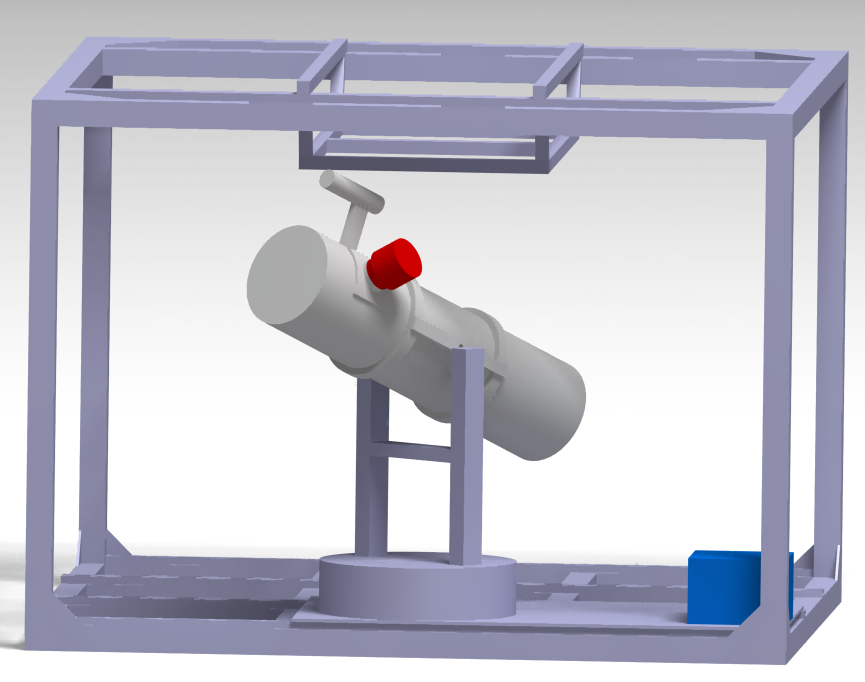
\includegraphics[scale=0.6]{figures/CAD/Assembly_1.png}
		\end{figure}
	\end{column}
	\begin{column}{0.3\textwidth}
		\begin{figure}
		\centering
		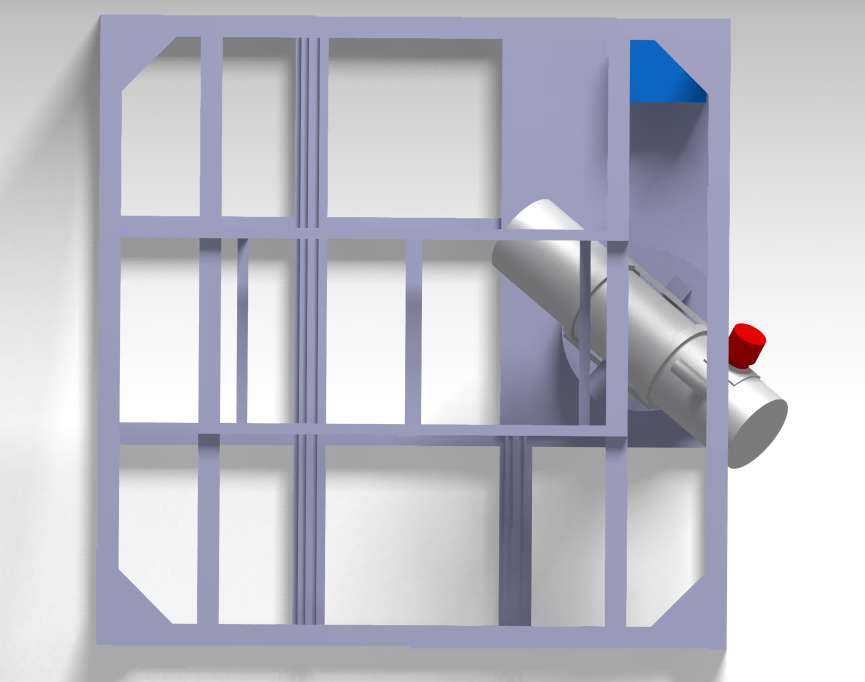
\includegraphics[scale=0.6]{figures/CAD/Assembly_2.png}
		\end{figure}
	\end{column}
	\begin{column}{0.3\textwidth}
		\begin{figure}
		\centering
		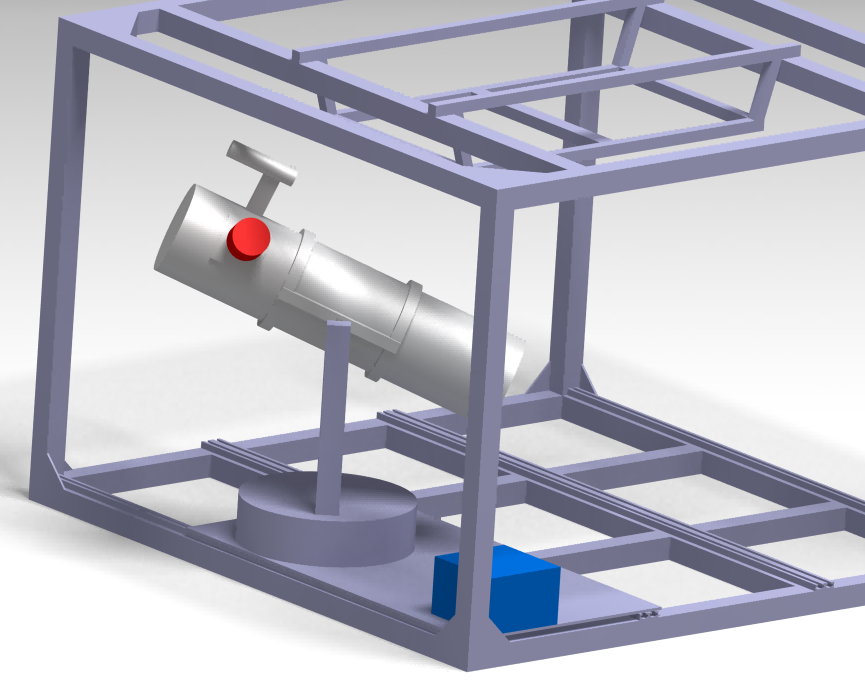
\includegraphics[scale=0.6]{figures/CAD/Assembly_3.png}
		\end{figure}
	\end{column}
\end{columns}
%Updated CAD design with the correct location and size. Would be a huge plus if it can rotate a bit.
\end{frame}

\subsection{Thermal} 			% DIEGO
\begin{frame}{Thermal}
\begin{itemize}
	\item Using a Newtonian telescope gives us the 				advantage of not needing an added baffle anymore since 			the 	primary mirror is situated on the rear part of the 		telescope, effectively using the telescope's structure 			as a baffle.
	\item For the electronics box, FEA analysis will be made in order to determine the heat produced by the components and therefore determine where heating or cooled will be required.
\end{itemize}

\end{frame}

\subsection{Electrical Setup}	% ELRICK
\begin{frame}[c]{Electrical ACD}
\centering
\begin{figure}
	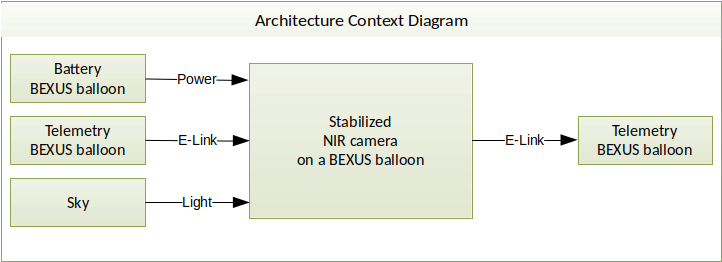
\includegraphics[width=1\textwidth]{figures/images/elec_ACD.png}
\end{figure}
\end{frame}

\begin{frame}{Electrical AID}
\begin{figure}
	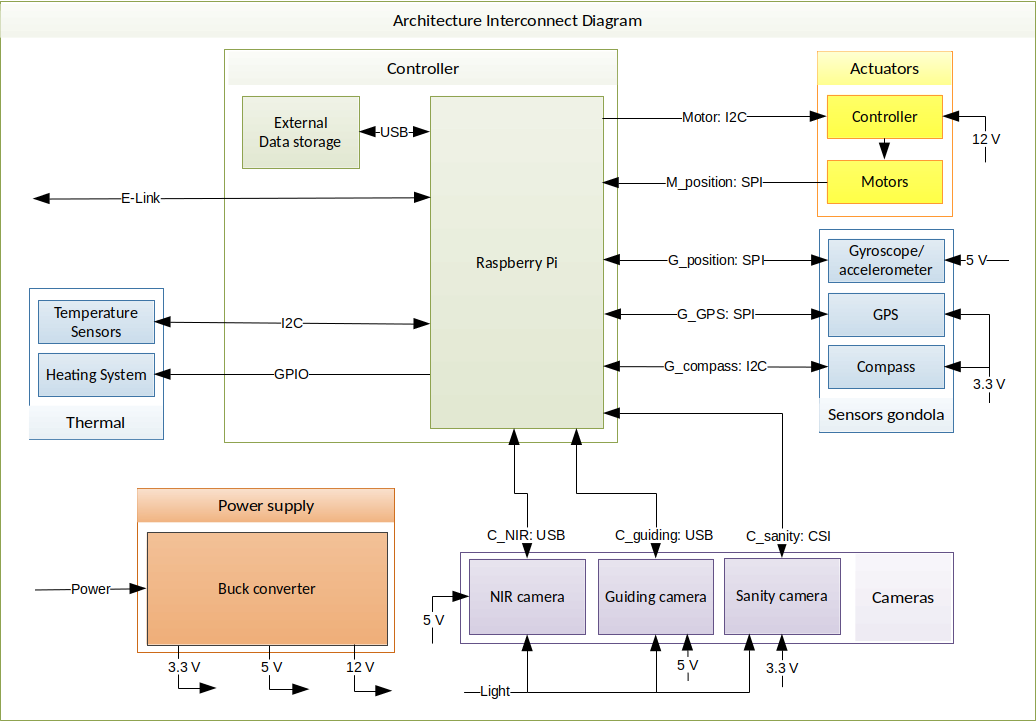
\includegraphics[width=.65\textwidth]{figures/images/elec_AID.png}
\end{figure}
\end{frame}

\begin{frame}{Power Consumption}
\centering
	\begin{tabular}{| l | l | l | l |}
	\hline
	& \textbf{Power [W]} & \textbf{On-time [\%]} & \textbf{Energy 4h [Wh]} \\\hline\hline
	NIR camera 		& 1.5	 	& 100 & 6 		\\\hline
	Guiding camera 	& 1.5 		& 100 & 6		\\\hline
	Controller 		& 6.25 		& 100 & 25		\\\hline
	Sensors 		& 1			& 100 & 4		\\\hline
	Motors			& 3 x 4.2	& 100 & 50.4	\\\hline
	Heating system 	& 10		& 20  & 8		\\\hline\hline
	
	Subtotal 		& & 			  & 99.4 Wh \\\hline\hline
	
	Standby E (6h) 	& & 			  & 40 Wh	\\\hline\hline
	
	Total			& & 			  & 139.4 Wh\\\hline
	\end{tabular}
\end{frame}

\begin{frame}[c]{Bandwidth}
\centering
\begin{tabular}{| l | l | l | l |}
	\hline
	\textbf{Item} & \textbf{File size*} & \textbf{Downlink rate} & \textbf{Datarate} \\\hline\hline
	
	NIR camera		& 18 MB & 60 sec 	& 2.4 Mbits/sec** \\\hline
	Guiding camera	& 2 MB	& 60 sec***	& 0.27 Mbits/sec \\\hline
	Sanity camera	& 7 MB  & On request & - \\\hline
	Sensors****		& 30 B  & 1 sec 	& 240 bits/sec \\\hline
	

\end{tabular}
\newline

\begin{columns}[t]
\begin{column}{0.1\textwidth}
\end{column}
\begin{column}{0.9\textwidth}
\begin{enumerate}
	\small
	\item[*] File sizes reflect lossless compressing
	\item[**] Not planned to send all pictures down, thus will be reduced
	\item[***] Onboard save time is 15 sec
	\item[****] GPS; Compass; Gyroscope; Encoders; NIR temp sensor
\end{enumerate}
\end{column}
\end{columns}
\end{frame}

\subsection{Ground Station} 	% NIKLAS
\begin{frame}{Ground Station}
\begin{itemize}
	\item K.I.S.S.
	\item Written in C with GTK+
\end{itemize}
\begin{figure}
	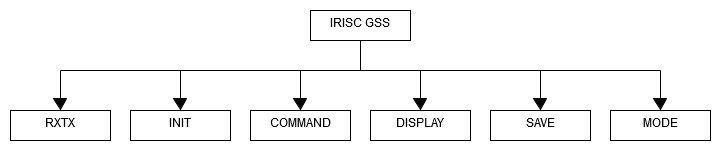
\includegraphics[scale=0.4]{figures/images/GSS-tree.png}
\end{figure}
\end{frame}

\subsection{OBSW} 	% NIKLAS
\begin{frame}{On-board Software}
\begin{itemize}
	\item The glue between the systems
	\item C on a simple linux distro
	\item Compression and storage
\end{itemize}
\begin{figure}
	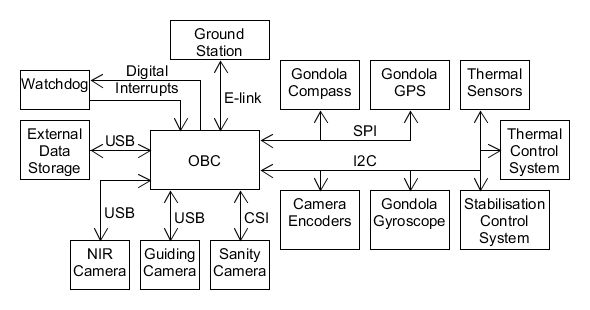
\includegraphics[scale=0.4]{figures/images/process-overview.png}
\end{figure}
\end{frame}

\subsection{Control System} 	% ANJA
\begin{frame}[t]{Control system}
\begin{itemize}
	\item<1-> Stabilisation of the gimbal: dynamic control system (e.\,g.~PID) \\
		Sensor data: gyroscopes, accelerometer\\
		Includes mechanical model of gimbal, motors
	\item<2-> Selection and tracking of targets: \\
		Sensor data: magnetometer, GPS, gyroscopes, encoders \\
		Includes model of movements of astronomical targets
	\item<3-> Feedback loop, measured states: utilisation of a Kalman filter to determine exact position \& orientation
\end{itemize}

\end{frame}

\begin{frame}[t]{Control system}
Minor objectives of the control system:
\begin{itemize}
	\item Avoid looking directly into the Sun
	\item Thermal control of the camera sensor and electronics
	\item Motor control
\end{itemize}

\end{frame}

\subsection{Cameras} 			% ANJA
\begin{frame}{NIR Camera}
\begin{columns}[t]
\begin{column}{0.6\textwidth}
	\begin{itemize}
		\item CMOS Sensor: ZWO ASI183MM (mono-colour) \\
			resolution: 20.18\,MP, sensor size: 13.2x8.8\,mm
		\item NIR-conversion with 720\,nm NIR filter
		\item Sensitivity: 720\,nm to 1150\,nm
		\item Rolling shutter: no mechanical shutter, no moving parts
	\end{itemize}
\end{column}
\begin{column}{0.4\textwidth}
	\begin{figure}[t]
		\centering
		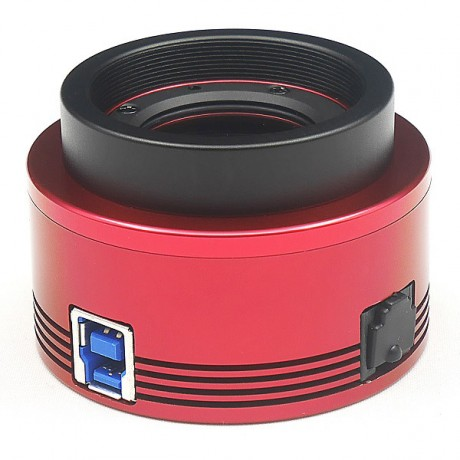
\includegraphics[width=0.7\linewidth]{figures/images/ZWO_ASI183MM.jpg}
		\caption*{Credits: ZWO ASI183MM (mono)}
		\label{fig::NIR_sensor}
	\end{figure}
\end{column}
\end{columns}
\end{frame}

\begin{frame}{Guiding Camera}
\begin{columns}[t]
\begin{column}{0.6\textwidth}
\begin{itemize}
	\item For verification of the field of view
	\item Support of ground-based re-calibration of sensors (e.\,g.~magnetometer, gyroscopes)
	\item Imaging sensor with a high sensitivity, resulting in shorter exposure times (compared to NIR camera)
	\item Imaging in visible wavelengths
\end{itemize}
\end{column}
\begin{column}{0.4\textwidth}
	\begin{figure}[t]
		\centering
		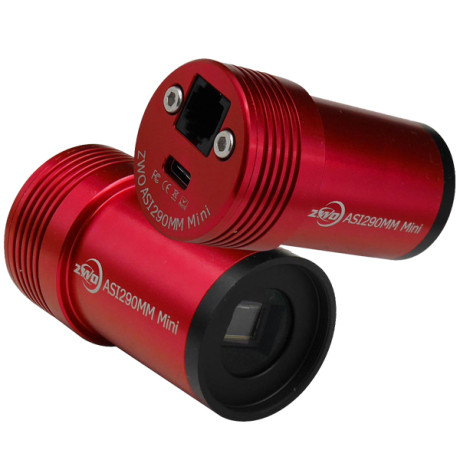
\includegraphics[width=0.7\linewidth]{figures/images/ZWO_ASI290MM_Mini.jpg}
		\caption*{Credits: Guiding camera by ZWO}
		\label{fig::guiding_camera}
	\end{figure}
\end{column}
\end{columns}
\end{frame}

%\begin{frame}{Sanity Camera}
%probably not going to be included in the presentation - any objections?
%\end{frame}

\subsection{Telescope} 			% KIM
\begin{frame}{Telescope}
\begin{figure}[!htb]
    \centering
    \begin{minipage}{.5\textwidth}
        \centering
        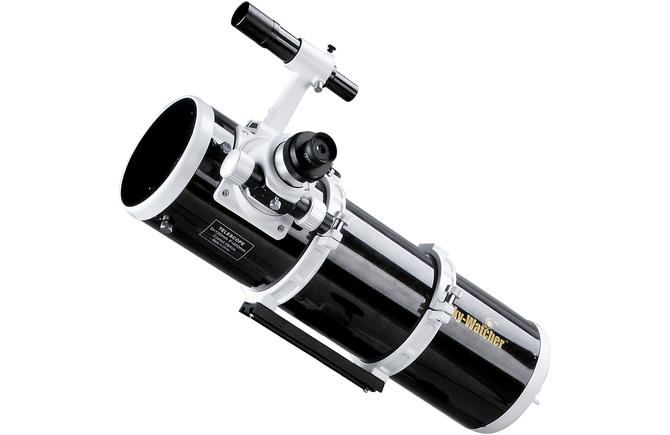
\includegraphics[width=0.9\linewidth]{figures/images/SkyWatcher_BKP130DS.jpg}
        \caption{Telescope (with eyepiece in place of the camera)}
    \end{minipage}%
    \begin{minipage}{0.5\textwidth}
    SkyWatcher BKP 130DS
    \begin{itemize}%[label=--]
        \item Newtonian telescope 
        \item Weight (without camera) 3.66\,kg
        \item Focal length: 650\,mm 
        \item Aperture: 130\,mm
        \item FOV: 1.16\,deg by 0.78\,deg (in combination with the camera)
        \item Diffraction-limited-resolution: 1.94\,arcsec
        \item Pixel size: 0.76\,arcsec (in combination with the camera)
    \end{itemize}
    \end{minipage}
\end{figure}
\end{frame}


%----------------------------------------------------------------------------------------
%	SCIENCE. 					  KIM
%----------------------------------------------------------------------------------------
\section{Science}
\subsection{Targets}
\begin{frame}{Targets}
\vspace{-0.25cm}
\begin{figure}[!htb]
    \begin{minipage}[t]{.42\textwidth}
        \centering
        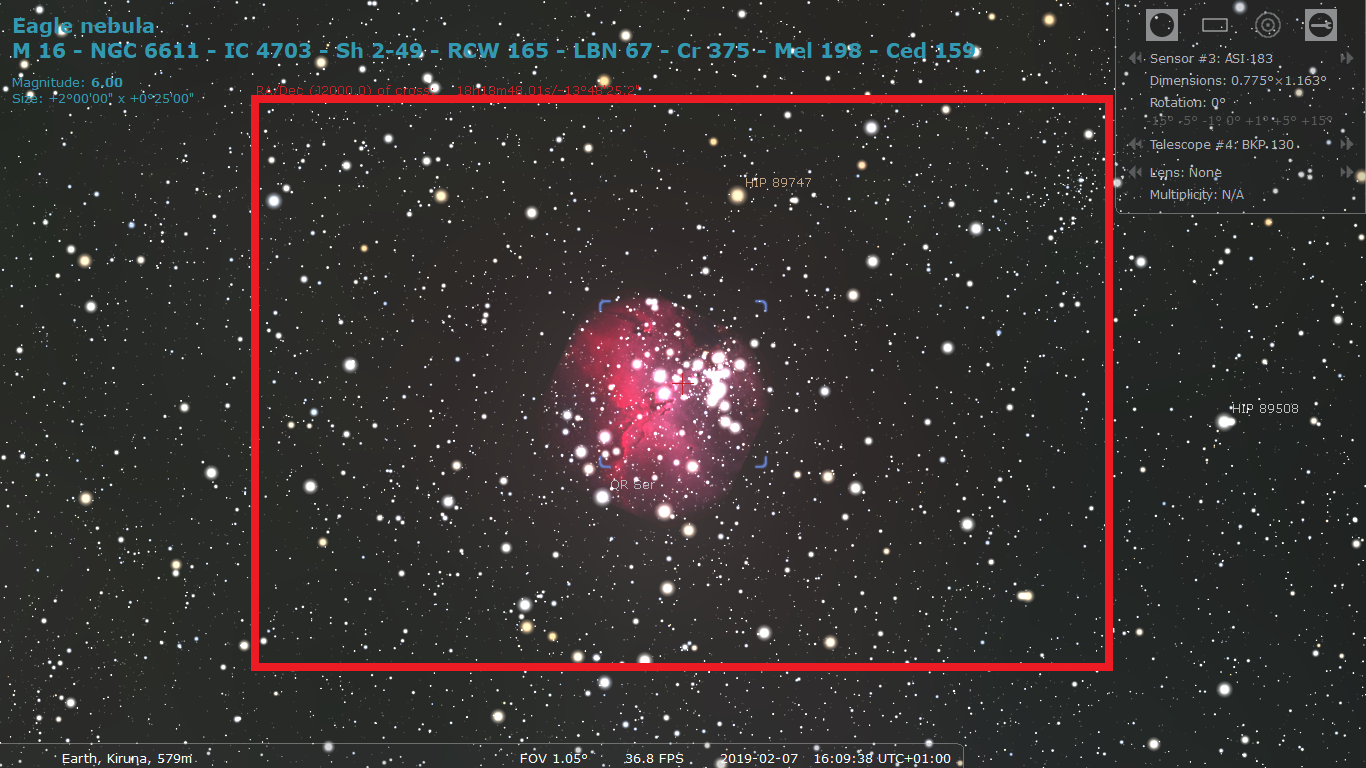
\includegraphics[width=\linewidth]{figures/targets/Eagle.png}
    \end{minipage}%
%    \hfill
	\begin{minipage}[t]{.42\textwidth}
        \centering
        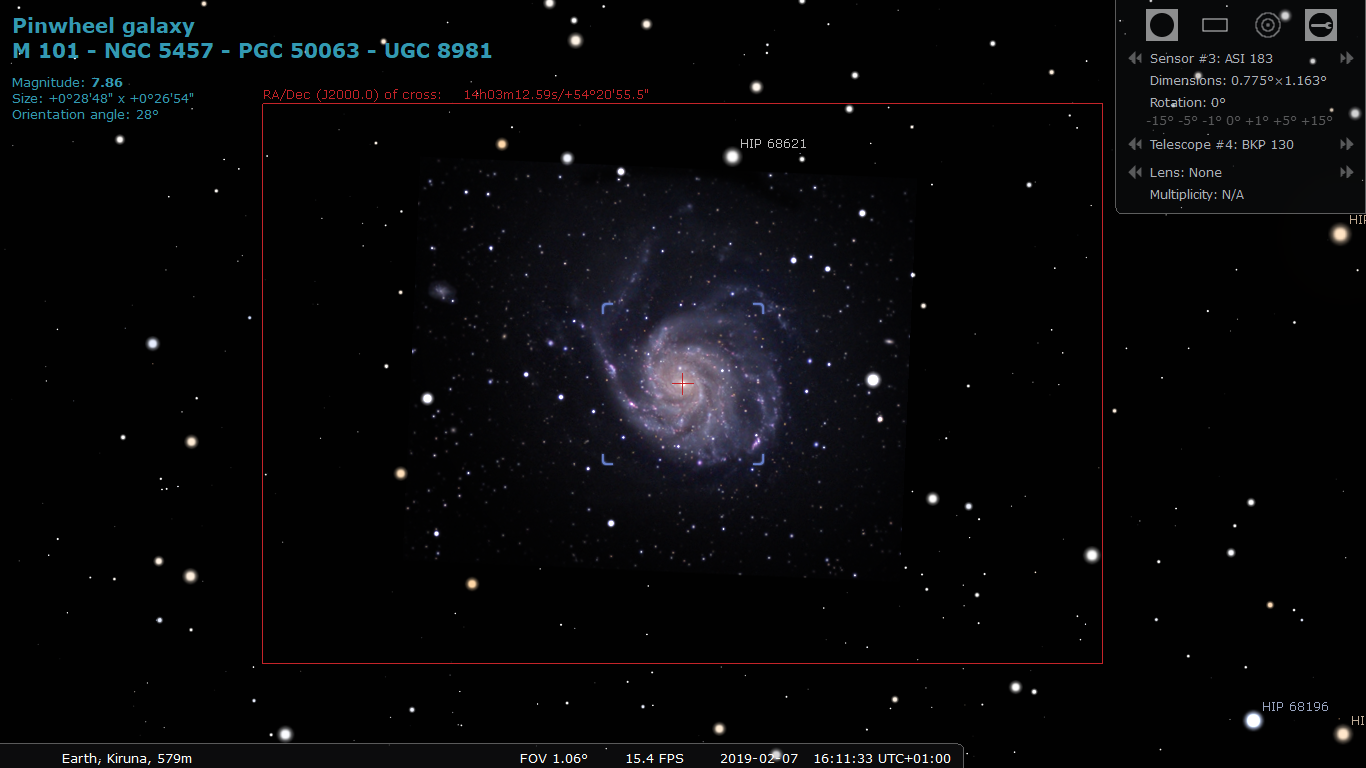
\includegraphics[width=\linewidth]{figures/targets/Pinwheel.png}
    \end{minipage}%
    
%    \medskip 
    
    \begin{minipage}[t]{.42\textwidth}
        \centering
        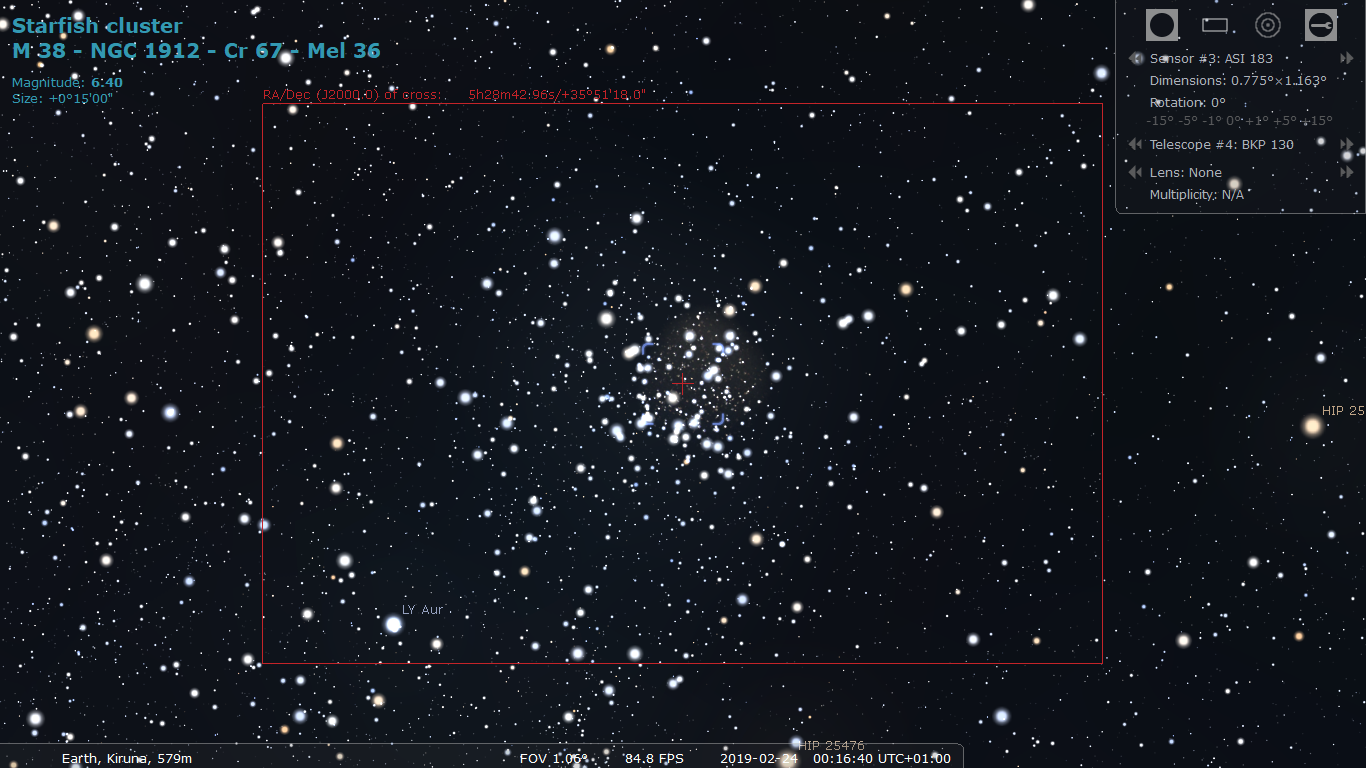
\includegraphics[width=\linewidth]{figures/targets/Starfish.png}
    \end{minipage}%
%    \hfill
    \begin{minipage}[t]{.42\textwidth}
        \centering
        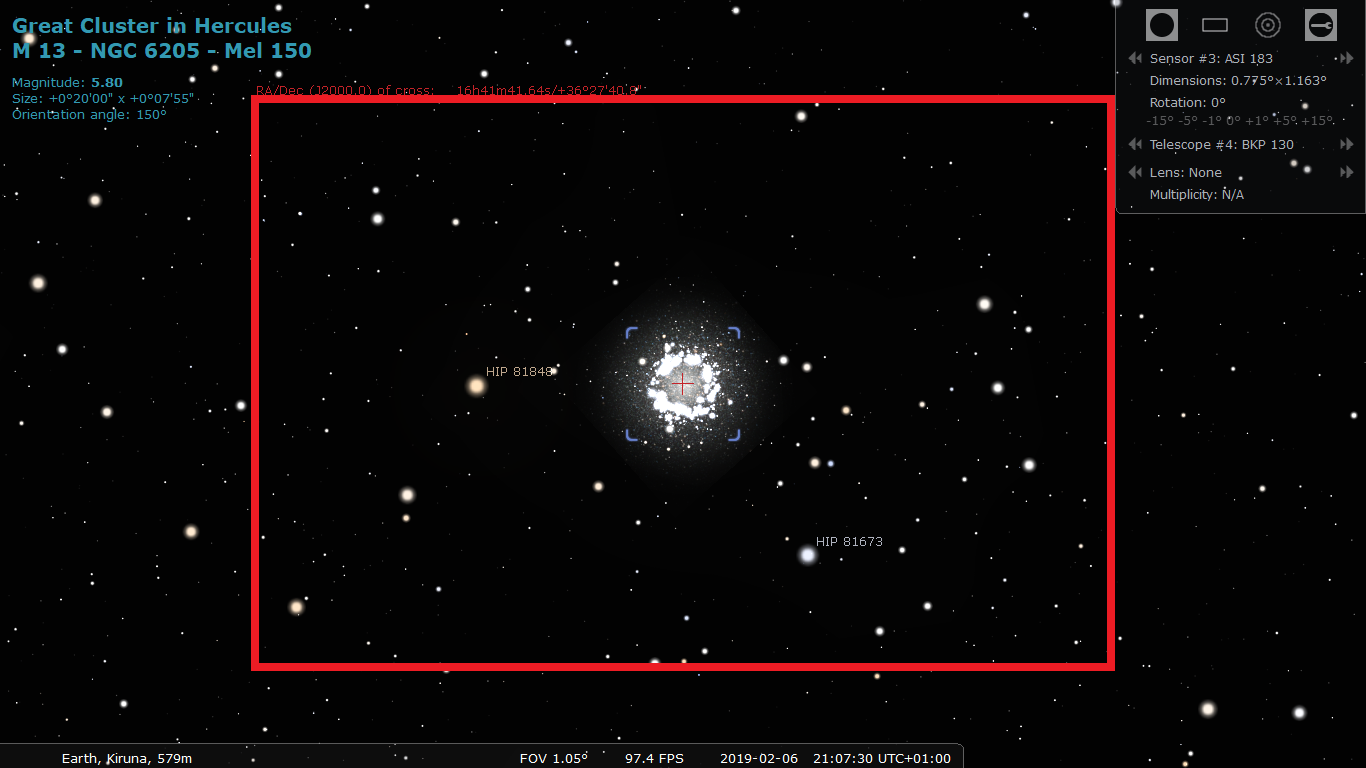
\includegraphics[width=\linewidth]{figures/targets/Hercules.png}
    \end{minipage}%
\end{figure}
\end{frame}

\subsection{Expected Results}
\begin{frame}{Signal to Noise Ratio}
\begin{figure}[!htb]
    \hspace{-2cm}
    \begin{minipage}{0.7\textwidth}
        \centering
        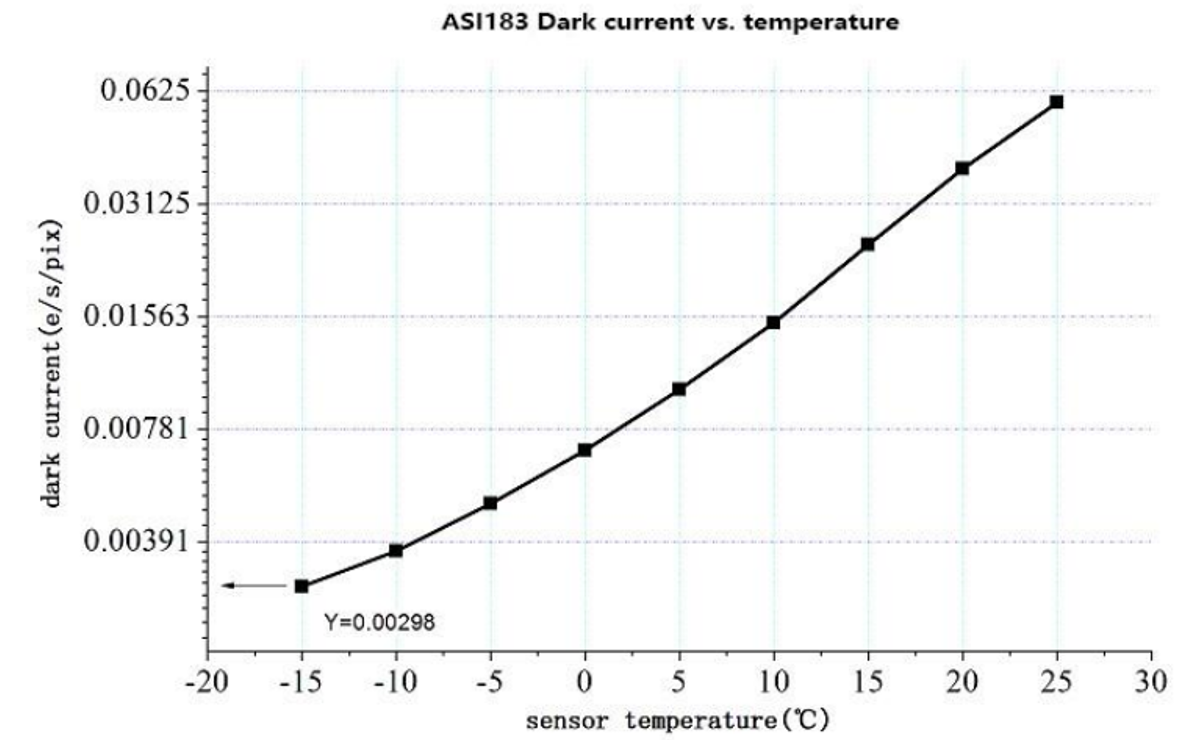
\includegraphics[width=0.8\linewidth]{figures/images/darkcurrent.PNG}
        \caption{Dark current vs. temperature as given in the camera manual}
    \end{minipage}%
    \begin{minipage}{0.3\textwidth}
	 	\centering
	 	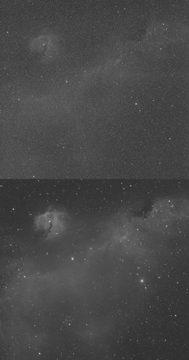
\includegraphics[width=0.8\linewidth]{figures/images/Uncool-189x360.jpg}
	 	\caption{Credit: Richard S. Wright Jr., SkyandTelescope.com}
    \end{minipage}
\end{figure}
\end{frame}

\subsection{Data Analysis}
\begin{frame}{Data Analysis}
\begin{figure}[!htb]
    \centering
    \begin{minipage}{0.7\textwidth}
        \centering
        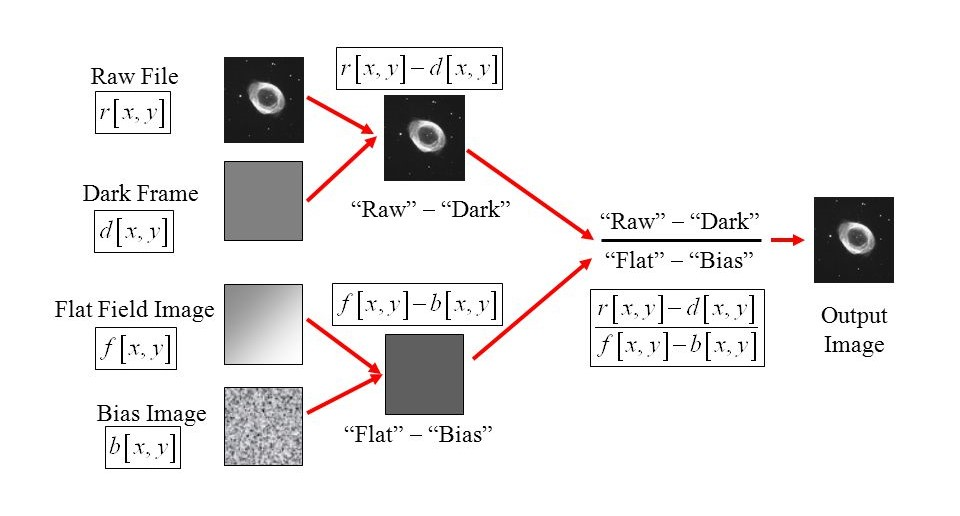
\includegraphics[width=0.9\linewidth]{figures/images/correctionpipeline.jpg}
        \caption{Standard astrophotography image calibration pipeline}
    \end{minipage}%
    \begin{minipage}{0.3\textwidth}
    \begin{itemize}%[label=--]
        \item \textbf{Light Frames:} image of the target itself.
        \item \textbf{Dark Frames:} aperture blocked of light.
        \item \textbf{Flat Frames:} brightness balance of the sensor
        \item \textbf{Bias Frames:} readout noise due to the sensor. 
    \end{itemize}
    \end{minipage}
\end{figure}
\end{frame}


%----------------------------------------------------------------------------------------
%	PROJECT MANAGEMENT.
%----------------------------------------------------------------------------------------
\section{Project Management}
\subsection{Schedule}
\nologo{
\begin{frame}{Schedule} 		% DIEGO
\begin{ganttchart}[
	hgrid,
	vgrid,
	expand chart=\textwidth,
	time slot format=isodate-yearmonth,
	time slot unit=month,
	y unit chart=.5cm,
	y unit title=.7cm
	]{2018-12}{2019-12}
	\gantttitle{BEXUS - IRISC}{13}\\
	\gantttitlecalendar{year, month=shortname} \\
	\ganttbar{Design Phase}{2018-12}{2019-04}\\
	\ganttbar{Unit testing}{2019-03}{2019-05}\\
	\ganttbar{Manufacturing Phase}{2019-04}{2019-07}\\
	\ganttmilestone {First Prototype}{2019-04}\\
	\ganttbar{Complete System Testing}{2019-06}{2019-09}\\
	\ganttbar{Launch Campaign}{2019-10}{2019-10}\\
	\ganttbar{Data Analysis Phase}{2019-11}{2019-12}
\end{ganttchart}

% global & zoomin
\end{frame}}

\subsection{Outreach} 			% NIKLAS
\begin{frame}{Outreach}
Website and Social media
\begin{itemize}
	\item Facebook
	\item Twitter
	\item Instagram
\end{itemize}
\end{frame}


%----------------------------------------------------------------------------------------
%	SUMMARY.
%----------------------------------------------------------------------------------------
\section{Summary}
\begin{frame}[t]{Summary} 		% ????
\centering
\begin{itemize}
    \item Proof of concept of a stabilised balloon-borne telescope with an NIR camera
    \item Empowered by the BEXUS project
    \item To achieve a higher degree of accessible and affordable astronomical research
    %\item Outreach to the public by website, social media, presentations, TV \& newspapers.
\end{itemize}

\begin{figure}
    \vspace{-.3cm}
    \subfloat{
        
\includegraphics[height=0.25\textwidth, valign=c]{figures/logos/IRISC_Black.png}
    } \hspace{2cm}
    \subfloat{
        
\includegraphics[height=0.25\textwidth, valign=c]{figures/logos/bexus.png}
    } 
\end{figure}
\end{frame}

\begin{frame}
    \centering
    \Huge Thank you for your attention\\\vspace{.3cm}
    \Large Let us explore the NIR universe with a BEXUS balloon together!\\
    
    %\huge Questions?\\\
    \vspace{1cm}
    \large \insertauthor \\\vspace{.2cm}%\insertauthor \\\vspace{.2cm}
    and the rest of the IRISC team
\end{frame}

%----------------------------------------------------------------------------------------
%	QUESTIONS.
%----------------------------------------------------------------------------------------
\section{Questions}
\begin{frame}
    \label{slide:questions}
    \centering
    \vspace{-0.71cm}
    \begin{figure}
    \hspace*{-1.1cm}
    	\includegraphics[width=1.15\textwidth]{figures/images/teamphoto.png}
    \end{figure}
\end{frame}

%----------------------------------------------------------------------------------------
%	BACKUP SLIDES. 				EVERYONE!!!
%----------------------------------------------------------------------------------------





%----------------------------------------------------------------------------------------
%	BACKUP SLIDES: 		ELECTRICAL
%----------------------------------------------------------------------------------------
\subsection{Electrical}
\begin{frame}[t]{Cooling electrical systems in space}
    The only way to get rid of thermal energy, outside the lower atmosphere, is radiation. Passive solutions are:
    \begin{itemize}
        \item Highly efficient components.
        \item Passive cooler with fluid (convection).
        \item Solid thermal conducting material connected to the heat sources (conduction).
    \end{itemize}
    
        \centering
        \vspace{1cm}
        \begin{figure}
            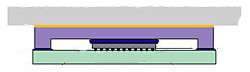
\includegraphics[width=.5\textwidth]{figures/images/Passive_cooler_2.jpg}\\
            \caption{Clemens J. M. Lasance, cooling electronics}
        \end{figure}
\end{frame}

\begin{frame}{Schematic: Sensors \& onboard computer}
	\vspace{-.2cm}
	\begin{figure}
		
\includegraphics[width=.68\textwidth]{figures/schematics/elec01.png}
	\end{figure}
\end{frame}

\begin{frame}{Schematic: Gyroscopes}
	\vspace{-.2cm}
	\begin{figure}
		
\includegraphics[width=.68\textwidth]{figures/schematics/elec02.png}
	\end{figure}
\end{frame}

\begin{frame}{Schematic: Motor Controller}
	\vspace{-.2cm}
	\begin{figure}
		
\includegraphics[width=.68\textwidth]{figures/schematics/elec03.png}
	\end{figure}
\end{frame}

\begin{frame}{Schematic: Thermal Sensors}
	\vspace{-.2cm}
	\begin{figure}
		
\includegraphics[width=.68\textwidth]{figures/schematics/elec04.png}
	\end{figure}
\end{frame}

\begin{frame}{Schematic: Heating System}
	\vspace{-.2cm}
	\begin{figure}
		
\includegraphics[width=.68\textwidth]{figures/schematics/elec05.png}
	\end{figure}
\end{frame}

\begin{frame}{Schematic: Power Management}
	\vspace{-.2cm}
	\begin{figure}
		
\includegraphics[width=.68\textwidth]{figures/schematics/elec06.png}
	\end{figure}
\end{frame}

%------------Control system - Anja-------------%

\subsection{Control System}
\begin{frame}[t]{Control System}
    \vspace{-0.5cm}
    \begin{figure}
        \centering
        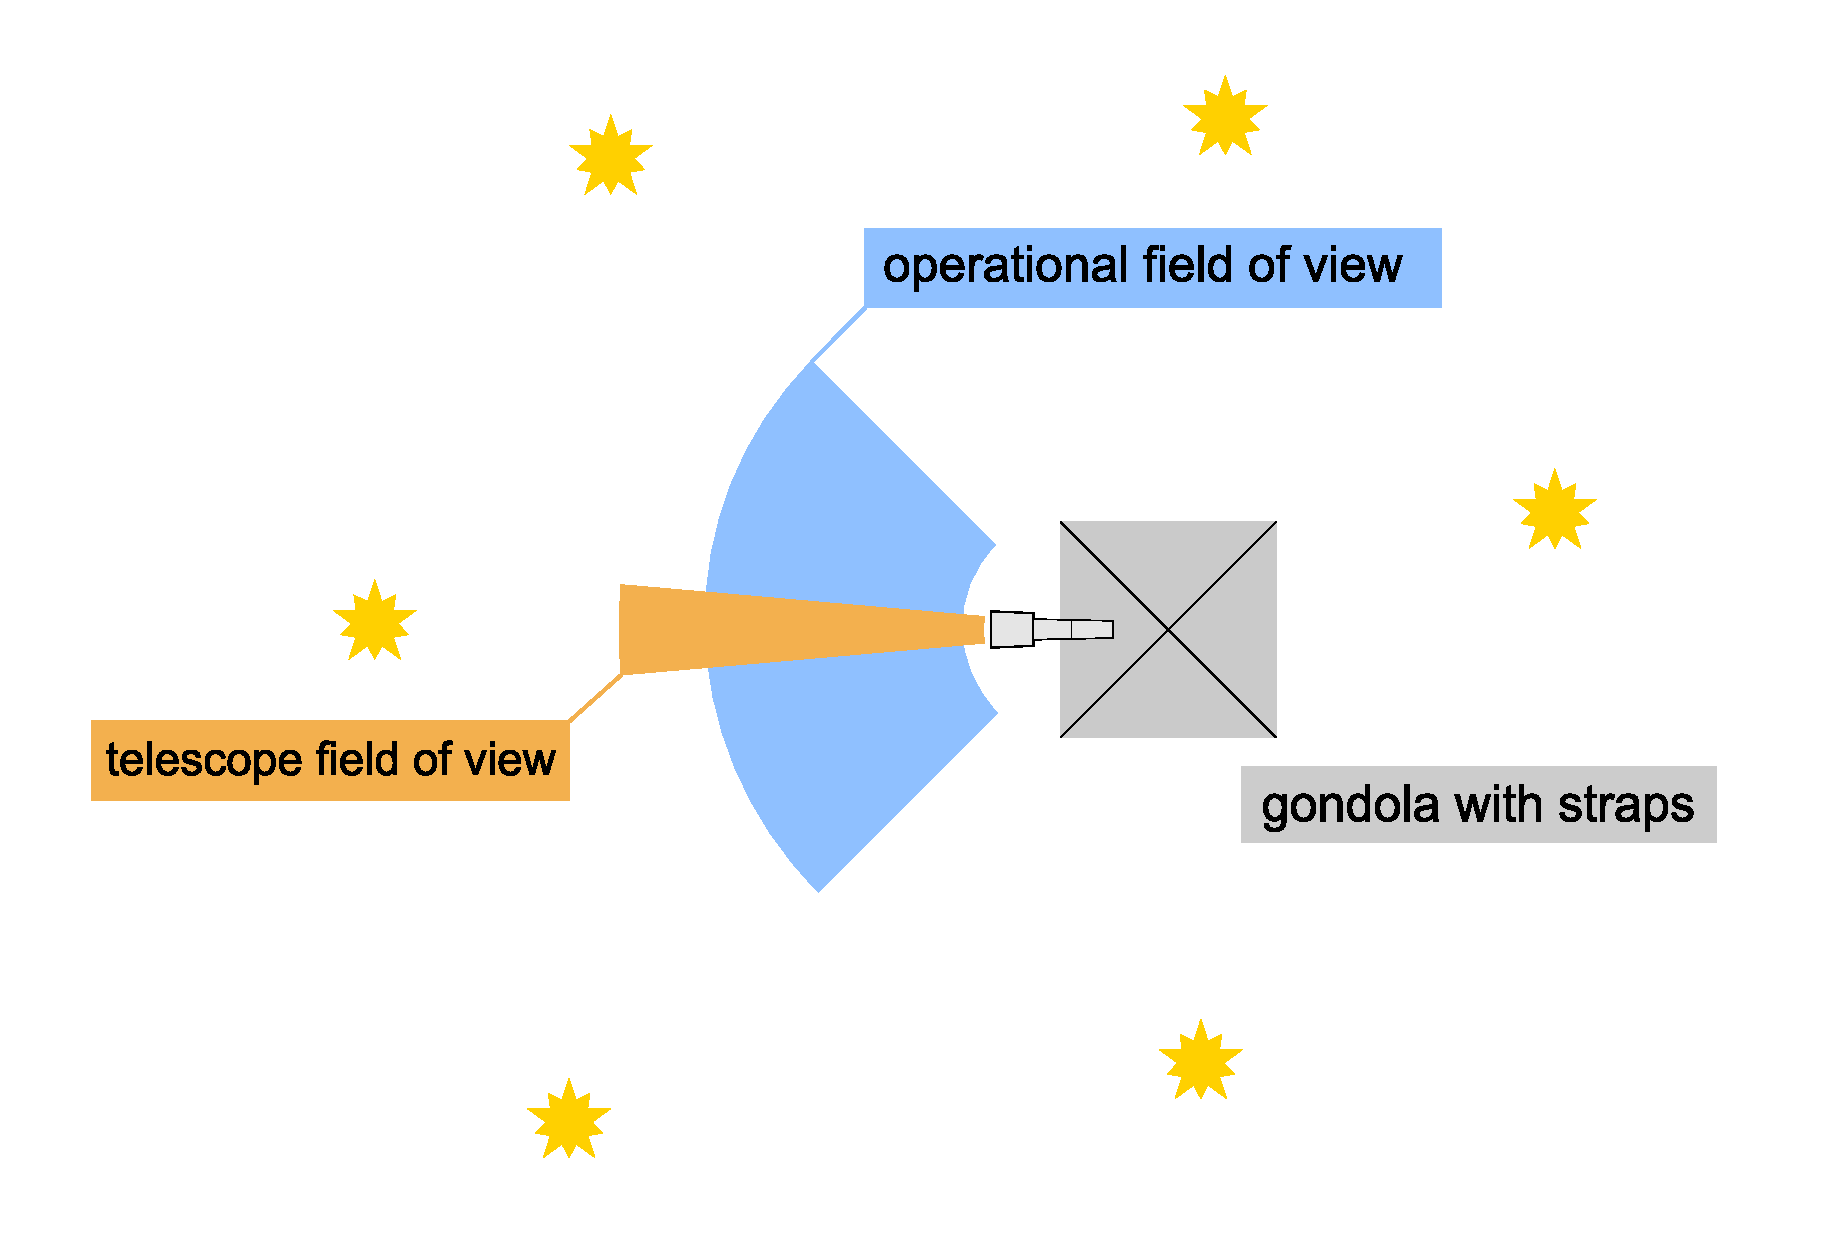
\includegraphics[width=0.7\textwidth]{figures/images/FoV_telescope.eps}
        \label{fig:FoV}
        %\caption*{Credit: https://publiclab.org/wiki/public-lab-lesson-3-photography-in-a-new-light}
    \end{figure}
\end{frame}

%------------Budget - Niklas-------------%

\subsection{Budget} 			% NIKLAS
\begin{frame}{Budget}
\begin{itemize}
	\item LTU Project funds
	\item Trusts and foundations
	\item Crowdfunding
\end{itemize}
\end{frame}

\end{document}
